% \documentclass[12pt, twoside]{book}
\documentclass[12pt, oneside]{book}  % jednostranna tlac
\usepackage[a4paper,top=2.5cm,bottom=2.5cm,left=3.5cm,right=2cm]{geometry}
\usepackage[utf8]{inputenc}
\usepackage[T1]{fontenc}
\usepackage{graphicx}
\usepackage{url}
\usepackage[hidelinks,breaklinks]{hyperref}
\usepackage{graphicx}
\usepackage[export]{adjustbox}
% \usepackage[slovak]{babel} % vypnite pre prace v anglictine
\linespread{1.25} % hodnota 1.25 by mala zodpovedat 1.5 riadkovaniu

% -------------------
% --- Definicia zakladnych pojmov
% --- Vyplnte podla vasho zadania
% -------------------
\def\mfrok{2018}
\def\mfnazov{Web teaching tool for learning agile programming}
\def\mftyp{Bachelor Thesis}
\def\mfautor{Tamara Savkova}
\def\mfskolitel{Ing. František Gyárfáš, CSc.}

%ak mate konzultanta, odkomentujte aj jeho meno na titulnom liste
% \def\mfkonzultant{tit. Meno Priezvisko, tit. }  

\def\mfmiesto{Bratislava, \mfrok}

% bioinformatici odkomentujú riadok s dvoma odbormi
\def\mfodbor{ 2511 Aplikovaná informatika }
%\def\mfodbor{ Informatika a Biológia } 
\def\program{ Aplikovaná informatika }
% Ak je školiteľ z FMFI, uvádzate katedru školiteľa, zrejme by mala byť aj na zadaní z AIS2
% Ak máte externého školiteľa, uvádzajte Katedru informatiky 
\def\mfpracovisko{ Department of Applied Informatics }

\begin{document}     
\frontmatter


% -------------------
% --- Obalka ------
% -------------------
\thispagestyle{empty}

\begin{center}
\sc\large
Comenius University in Bratislava\\
Faculty of Mathematics, Physics and Informatics

\vfill

{\LARGE\mfnazov}\\
\mftyp
\end{center}

\vfill

{\sc\large 
\noindent \mfrok\\
\mfautor
}

\cleardoublepage
% --- koniec obalky ----

% -------------------
% --- Titulný list
% -------------------

\thispagestyle{empty}
\noindent

\begin{center}
\sc  
\large
Comenius University in Bratislava\\
Faculty of Mathematics, Physics and Informatics

\vfill

{\LARGE\mfnazov}\\
\mftyp
\end{center}

\vfill

\noindent
\begin{tabular}{ll}
Program of Study: & \program \\
Field of Study: & \mfodbor \\
Department: & \mfpracovisko \\
Supervisor: & \mfskolitel \\
\end{tabular}

\vfill


\noindent \mfmiesto\\
\mfautor

\cleardoublepage
% --- Koniec titulnej strany


% -------------------
% --- Zadanie z AIS
% -------------------
% v tlačenej verzii s podpismi zainteresovaných osôb.
% v elektronickej verzii sa zverejňuje zadanie bez podpisov
% v pracach v anglictine anglicke aj slovenske zadanie

\newpage 
\thispagestyle{empty}
\hspace{-2cm}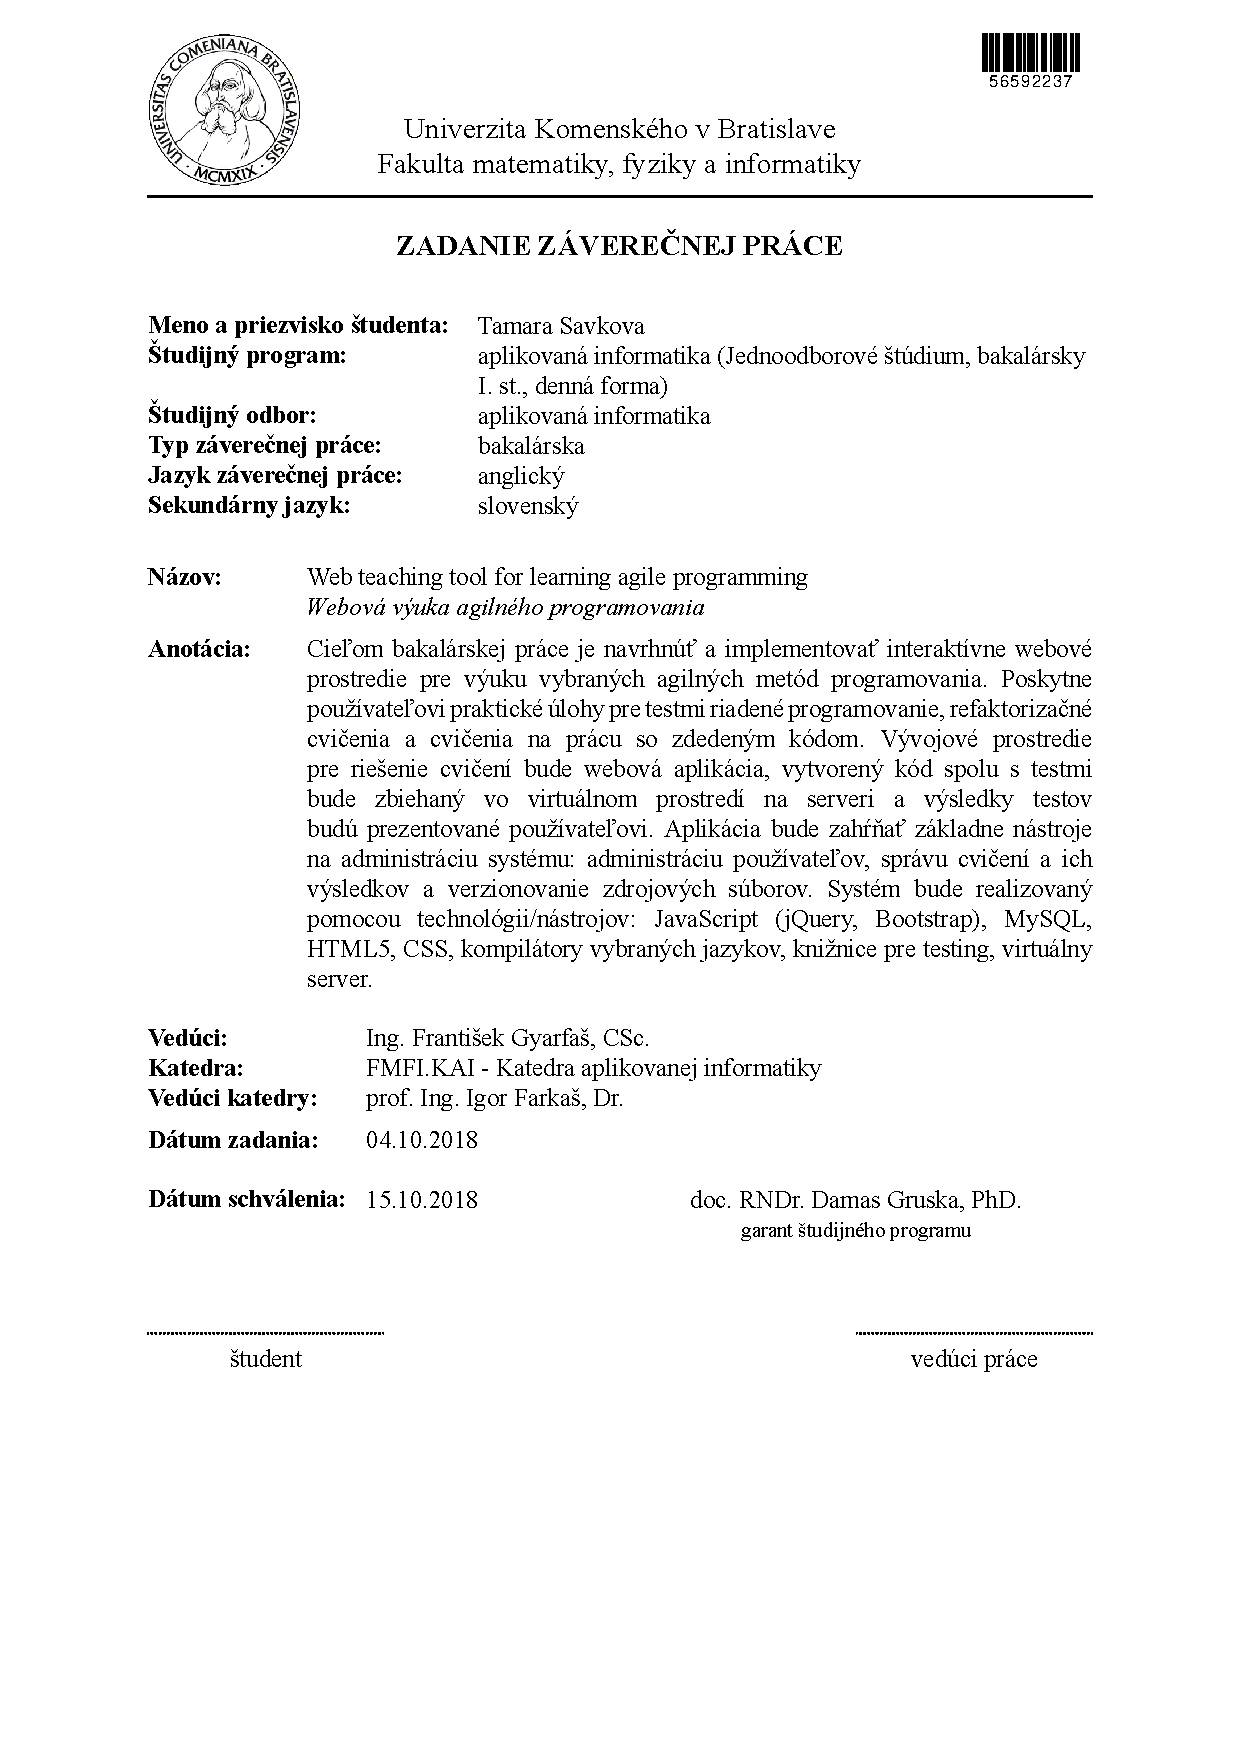
\includegraphics[width=1.1\textwidth]{images/zadanie}

% --- Koniec zadania

\frontmatter

% -------------------
%   Poďakovanie - nepovinné
% -------------------
\setcounter{page}{3}
\newpage 
~

% \vfill
% {\bf Poďakovanie:} Tu môžete poďakovať školiteľovi, prípadne
% ďalším osobám, ktoré vám s prácou nejako pomohli, poradili,
% poskytli dáta a podobne.

% --- Koniec poďakovania

% -------------------
%   Abstrakt - Slovensky
% -------------------
\newpage 
\section*{Abstrakt}


Cieľom bakalárskej práce je navrhnúť a implementovať interaktívne webové prostredie pre výuku vybraných agilných metód programovania. Poskytne používateľovi praktické úlohy pre testmi riadené programovanie, refaktorizačné cvičenia a cvičenia na prácu so zdedeným kódom. Vývojové prostredie pre riešenie cvičení bude webová aplikácia, vytvorený kód spolu s testmi bude zbiehaný vo virtuálnom prostredí na serveri a výsledky testov budú prezentované používateľovi. Aplikácia bude zahŕňať základne nástroje na administráciu systému: administráciu používateľov, správu cvičení a ich výsledkov a verzionovanie zdrojových súborov. Systém bude realizovaný pomocou technológii/nástrojov: JavaScript (jQuery, Bootstrap), MySQL, HTML5, CSS, kompilátory vybraných jazykov, knižnice pre testing, virtuálny server.

\paragraph*{Kľúčové slová:} webová alikacia, testami riadený vývoj, zdenený kód, čistý kód, refaktorizácia, edukačný softvér.
% --- Koniec Abstrakt - Slovensky


% -------------------
% --- Abstrakt - Anglicky 
% -------------------
\newpage 
\section*{Abstract}

The aim of the bachelor thesis is to design and implement an interactive web environment for the teaching of selected agile programming methods. It provides the user with practical tasks for test-driven development, exercises on refactoring and working with legacy code. The web application will be the development environment, the generated code along with the tests will be run in the virtual environment on the server and the test results will be presented to the user. The application will include basic system administration tools: users administration, managing the exercises and their results, and source code version control. The system will be implemented using technologies/tools: JavaScript (jQuery, Bootstrap), MySQL, HTML5, CSS, compilers of selected languages, testing libraries, virtual server.


\paragraph*{Keywords:} web application, test-driven development, legacy code, clean code, refactoring, educational software.

% --- Koniec Abstrakt - Anglicky

% -------------------
% --- Predhovor - v informatike sa zvacsa nepouziva
% -------------------
%\newpage 
%\thispagestyle{empty}
%
%\huge{Predhovor}
%\normalsize
%\newline
%Predhovor je všeobecná informácia o práci, obsahuje hlavnú charakteristiku práce 
%a okolnosti jej vzniku. Autor zdôvodní výber témy, stručne informuje o cieľoch 
%a význame práce, spomenie domáci a zahraničný kontext, komu je práca určená, 
%použité metódy, stav poznania; autor stručne charakterizuje svoj prístup a svoje 
%hľadisko. 
%
% --- Koniec Predhovor


% -------------------
% --- Obsah
% -------------------

\newpage 

\tableofcontents

% ---  Koniec Obsahu

% -------------------
% --- Zoznamy tabuliek, obrázkov - nepovinne
% -------------------

\newpage 

\listoffigures
\listoftables

% ---  Koniec Zoznamov

\mainmatter


\input content/intro.tex 

\input content/sources.tex

\input content/concept.tex

\input content/implementation.tex

\input content/sample_course.tex

\input content/conclusion.tex

% -------------------
% --- Bibliografia
% -------------------


\newpage	

\backmatter

\thispagestyle{empty}
\nocite{*}
\clearpage

\bibliographystyle{plain}
\bibliography{literature/lit_sources,literature/lit_concept,literature/lit_implementation}

%Prípadne môžete napísať literatúru priamo tu
%\begin{thebibliography}{5}
 
%\bibitem{br1} MOLINA H. G. - ULLMAN J. D. - WIDOM J., 2002, Database Systems, Upper Saddle River : Prentice-Hall, 2002, 1119 s., Pearson International edition, 0-13-098043-9

%\bibitem{br2} MOLINA H. G. - ULLMAN J. D. - WIDOM J., 2000 , Databasse System implementation, New Jersey : Prentice-Hall, 2000, 653s., ???

%\bibitem{br3} ULLMAN J. D. - WIDOM J., 1997, A First Course in Database Systems, New Jersey : Prentice-Hall, 1997, 470s., 

%\bibitem{br4} PREFUSE, 2007, The Prefuse visualization toolkit,  [online] Dostupné na internete: <http://prefuse.org/>

%\bibitem{br5} PREFUSE Forum, Sourceforge - Prefuse Forum,  [online] Dostupné na internete: <http://sourceforge.net/projects/prefuse/>

%\end{thebibliography}

%---koniec Referencii

% -------------------
%--- Prilohy---
% -------------------

%Nepovinná časť prílohy obsahuje materiály, ktoré neboli zaradené priamo  do textu. Každá príloha sa začína na novej strane.
%Zoznam príloh je súčasťou obsahu.
%
%\addcontentsline{toc}{chapter}{Appendix A}
%\input AppendixA.tex
%
%\addcontentsline{toc}{chapter}{Appendix B}
%\input AppendixB.tex

\end{document}






